\documentclass{article}

\usepackage{microtype}
\usepackage{graphicx}
\usepackage{booktabs}
\usepackage{hyperref}
\newcommand{\theHalgorithm}{\arabic{algorithm}}
\usepackage{icml2026}
\usepackage{algorithm}
\usepackage{algorithmic}

\usepackage{amsmath,amssymb,mathtools,amsthm}
\usepackage[shortlabels]{enumitem}
\usepackage{xcolor}
\usepackage{float}
\usepackage[capitalize,noabbrev]{cleveref}

\theoremstyle{plain}
\newtheorem{theorem}{Theorem}[section]
\newtheorem{proposition}[theorem]{Proposition}
\newtheorem{lemma}[theorem]{Lemma}
\newcommand{\E}{\mathbb E}
\graphicspath{{figures/}{../../docs/figures/}}
\newcommand{\pending}[1]{\textcolor{red}{[#1]}}

\icmltitlerunning{RLVR Moves Along a Coverage Frontier Set by the Base Model}
\makeatletter\newcommand{\setrunninghead}{\gdef\@icmltitlerunning{RLVR Moves Along a Coverage Frontier Set by the Base Model}}\makeatother

\begin{document}

\twocolumn[
  \icmltitle{RLVR Moves Along a Coverage Frontier Set by the Base Model:\\
  Pre-Registered Evidence from RL Interventions, Warm Starts and Public Checkpoints}
  \setrunninghead
  \begin{icmlauthorlist}
    \icmlauthor{Anonymous Authors}{anon}
  \end{icmlauthorlist}
  \icmlaffiliation{anon}{Anonymous Institution}
  \icmlcorrespondingauthor{Anonymous Authors}{anon@anon}
  \icmlkeywords{reinforcement learning with verifiable rewards, pass@k, diversity, exploration, warm start, evaluation}
  \vskip 0.3in
]
\printAffiliationsAndNotice{}

\begin{abstract}
Many methods claim to make reinforcement learning with verifiable rewards (RLVR) more diverse, usually by reporting
higher pass@$k$ at a fixed number of training steps. A method that learns more slowly is less sharpened at any fixed
step, so such comparisons mix speed with coverage. We compare pass@16 at matched pass@1, with decision rules
registered before each run and problem-bootstrap intervals. On Qwen2.5-Math-1.5B and 7B, the interpretable
comparisons of more than twenty RL-side interventions---advantage rules, two outcome-diversity bonuses,
sharpness-aware updates, replay, larger groups, rollout allocation, guidance prefixes and 1,000-step training---are
consistent with movement along Dr.\ GRPO's pass@16-versus-pass@1 curve, not with a change of the curve, and 26 public
checkpoints from other groups fall on or below a curve predicted from the base model. Small supervised warm starts
before RL are the only lever we found that lifts the curve: teacher solutions raise matched pass@16 by $+2.1$ points
over early RL, beat the base model's own solutions on identical prompts ($+1.53$, 95\% $[+0.34,+2.76]$), and keep
their effect with corrupted final answers; coverage weighting, TailSFT-style filtering, hard-only selection and
interleaving the same data during RL do not add to this. Against 700-step Dr.\ GRPO references, however, every start's
advantage decays to about $+0.4$ points by step 150 (three seeds, descriptive): starts accelerate progress along the
frontier and make a transient excursion above it. Per-problem decompositions locate teacher gains on problems the base model never
solves. We conclude that, in these settings, RLVR's coverage at a given accuracy is a property of the starting model,
and we outline what a method would have to do to change it.
\end{abstract}

\section{Introduction}
RLVR trains a language model on automatically checked answers \citep{shao2024deepseekmath,guo2025r1}. Because RL
sharpens the policy, RL-trained models are often beaten by their own base model at large $k$ \citep{yue2025limit},
and a growing literature tries to keep rollouts diverse: modified advantages \citep{zhu2025nsr,walder2025pkpo,
chen2025passktraining}, exploration bonuses \citep{song2025outcome}, entropy control \citep{cui2025entropy}, rollout
budgets \citep{hu2025brorl,yang2025depth,knapsack2025,yu2026datpo}, off-policy guidance \citep{yan2025guidance,
ma2025relift,li2025questa,zhang2025bread} and warm starts \citep{dong2026opd,malladi2026tailsft}. Most report pass@$k$
at a fixed step.

We separate speed from coverage by comparing a method's pass@16 with a reference curve at the \emph{same pass@1}
(\cref{sec:setup}). Every decision rule is registered before its run; intervals resample test problems and recompute
the reference in each draw. Our findings:
\begin{enumerate}[leftmargin=*,itemsep=1pt,topsep=2pt]
\item \textbf{RL-side interventions stay on one curve} (\cref{sec:rl}): more than twenty registered interventions,
including the outcome-based exploration bonuses of \citet{song2025outcome} and sharpness-aware Flat-RLVR
\citep{kim2026flat}, reach average equivalence with Dr.\ GRPO's curve or remain within $\pm1.2$ points; 1,000-step
training raises pass@1 by 9--13 points without meeting the registered coverage criterion.
\item \textbf{Public checkpoints lie on or below the base-predicted curve} (\cref{sec:public}): 26 checkpoints, 38
evaluations, largest residual $+0.9$ points.
\item \textbf{Warm starts lift the curve during early RL, and teacher content is what matters}
(\cref{sec:starts}): teacher-solution starts meet the registered curve-raised criterion, beat the base model's own
solutions on identical, length-matched prompts, and survive corrupted final answers; how the SFT data is weighted,
filtered or timed does not matter.
\item \textbf{The excursion is transient} (\cref{sec:persist}): against 700-step references, all start advantages
decay by RL step 150, while teacher starts reach the 700-step reference's accuracy in 150 steps.
\item \textbf{Where gains sit} (\cref{sec:where}): matched-accuracy coverage gains are across-problem spread (pass@2),
and teacher gains concentrate on problems with zero base successes; self-generated starts gain on problems the base
already solves sometimes, where RL catches up.
\end{enumerate}

\section{Setup and protocol}\label{sec:setup}
For problem $x$ with binary reward, $p_x$ is the policy's success probability. Over $N$ problems,
$P_k=\frac1N\sum_x[1-(1-p_x)^k]$, estimated without bias from $n_x$ samples with $C_x$ successes
\citep{chen2021codex}.

\begin{proposition}[pass@$k$ at matched pass@1 measures spread]\label{prop:spread}
$P_1=\E_xp_x$ and $P_k=\E_xf_k(p_x)$ with $f_k(p)=1-(1-p)^k$ strictly concave for $k>1$. At fixed mean, a
mean-preserving spread of $\{p_x\}$ lowers $P_k$; in particular $P_2=2P_1-\E_xp_x^2$, so at matched pass@1 the
pass@2 gap equals minus the change in the second moment of success across problems. For a small change $\delta_x$ with
$\E\delta_x=0$, the first-order pass@$k$ change is $\mathrm{Cov}_x\big(k(1-p_x)^{k-1},\delta_x\big)$.
\end{proposition}

\textbf{Training.} Dr.\ GRPO \citep{liu2025drgrpo}: group-relative advantages $r_i-\bar r$, sequence-sum loss with a
constant normalizer, one update per batch of fresh rollouts, no KL term, AdamW at $10^{-6}$, 16 problems $\times$ 8
rollouts per step, 150 steps, MATH training problems \citep{hendrycks2021math}. Qwen2.5-Math-1.5B
\citep{yang2024qwen25math} at 512 or 1,024 response tokens; 7B at 2,048 tokens. Reference runs (B1k, three seeds)
used one L40S each; warm-start arms used A100s (\cref{sec:limits}).

\textbf{Evaluation.} 511 held-out MATH test problems, 32 samples at $T=1$ (64 for starting models, 256 where stated),
vLLM with per-problem seeds and the training prompt.

\textbf{Matched-accuracy estimator.} For a checkpoint with pass@1 $a$, the gap is $\widehat P_{16}-R_s(a)$, where $R_s$
is the same-seed reference trajectory (base and saved steps, sorted by pass@1) linearly interpolated at $a$.
Eligible checkpoints have $a$ inside $R_s$'s range on the full data; a seed needs two. Gaps average eligible
checkpoints within a seed, then seeds equally. 2,000 problem-bootstrap draws recompute the reference; from
Pre-registration 36 on, the checkpoint set is fixed and a seed's draw is unavailable if any checkpoint leaves the
reference's range, and a seed with more than 10\% unavailable draws makes the contrast ``not interpreted (support)''.
\emph{Curve raised}: pooled gap $\ge+2$, 95\% interval above 0, every seed positive, Holm $p\le0.05$.
\emph{Average equivalence}: pooled (and, from Pre-registration 20, each seed's) 90\% interval within $\pm2$.
\emph{Arm beats arm} (method contrasts, one arm's checkpoints against the other's trajectory): pooled $\ge+0.5$, 95\%
interval above 0, every seed positive, Holm $p\le0.05$. Intervals condition on the trained seeds.

\section{RL-side interventions stay on one curve}\label{sec:rl}
\Cref{tab:rl} collects registered comparisons. Advantage rules (PSR, NSR, constant baselines, noise injection, pass@$k$
objectives, MaxRL), entropy terms, replay and group completion, larger groups (32 rollouts), rollout allocation by
frontier value and its controls, human-solution and self-generated prefix guidance, process credit, update-geometry
changes and sharpness-aware updates either reach average equivalence or stay within $\pm1.2$ points with intervals
including zero; full verdicts are in \cref{app:prereg}. The UCB-Con bonus raises distinct valid incorrect answers per
problem by $0.057$ (its registered diversity rule) without moving the curve ($+0.40$); its matched pass@32 gap
($+0.31$, 95\% $[-0.25,+0.78]$) excludes the $+1.7$-point magnitude reported by \citet{song2025outcome}, whose
training, model and implementation differ. Allocation by frontier value raises the share of success-bearing groups
among pilot-zero problems from 18--21\% to 50--54\% and still stays on the curve (forecast $+4.1$, observed $-0.05$):
lack of on-policy signal on rare problems is not, in this form, what fixes the curve.

\begin{table}[t]
\caption{Registered matched-pass@1 differences in pass@16 (points; 95\% intervals unless marked 90\%). Reference:
Dr.\ GRPO (B) trajectory or trajectory-and-temperature envelope. 1.5B unless stated.}
\label{tab:rl}
\centering\small
\resizebox{\columnwidth}{!}{\begin{tabular}{@{}llr@{}}
\toprule
Comparison & Setting & Difference\\
\midrule
NSR vs PSR & 512 tok., 3 seeds & $-0.20$ [$-0.97$, $+0.55$] (90\%)\\
Coverage-weighted replay vs B & 512, 3 seeds & $+1.19$ [$+0.54$, $+1.79$]\\
Allocation (frontier value) vs B & 1,024, 3 seeds & $-0.12$ [$-0.60$, $+0.29$]\\
PSR / NSR vs B & 1,024, 3 seeds & $+0.11$ / $-0.15$\\
Human / self prefixes vs B & 1,024, 3 seeds & $-0.05$ / $-0.11$\\
UCB-Con bonus vs B & 1,024, 3 seeds & $+0.40$ [$+0.02$, $+0.76$]\\
Batch bonus vs B & 1,024, 3 seeds & $+0.01$ [$-0.38$, $+0.39$]\\
Flat-RLVR ($\rho$ 10 / 5) vs B & 1,024, 3 seeds & $+0.29$ [$-0.09$, $+0.69$] / $-0.02$\\
PSR / NSR / allocation vs B & 7B, 2,048, 2 seeds & $-0.09$ / $-0.09$ / $-0.15$ (90\%)\\
\bottomrule
\end{tabular}}
\end{table}

\begin{figure}[t]
\centering
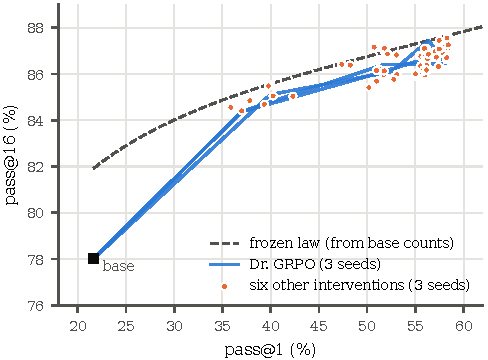
\includegraphics[width=\columnwidth]{curve_1k.pdf}
\caption{1.5B at 1,024 tokens: Dr.\ GRPO trajectories (three seeds) and checkpoints of six interventions (three seeds
each). Dashed: a frozen per-problem law computed from the base model's success counts (\cref{app:law}).}
\label{fig:curve}
\end{figure}

\textbf{Longer training.} Dr.\ GRPO for 1,000 steps at learning rates $10^{-6}$ and $3\times10^{-6}$ raises pass@1
from $57.8$ to $67.2$ and from $63.7$ to $70.7$; pass@256 at step 1,000 minus the base is $+1.96$ [$+0.39$, $+3.72$]
and $+0.39$ [$-1.37$, $+2.15$], with Holm-adjusted one-sided $p=0.029$ and $0.358$ against the registered $0.025$:
not supported, the first borderline (\cref{fig:long}). The base model's difficulty order is largely preserved
(Spearman $0.67$--$0.72$).

\begin{figure}[t]
\centering
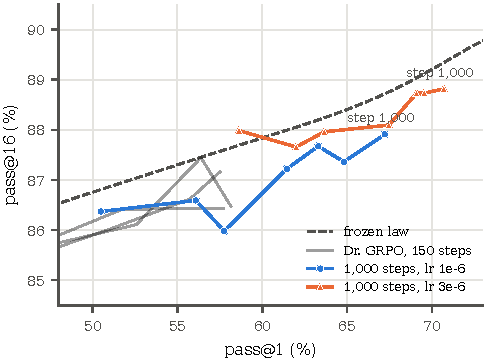
\includegraphics[width=\columnwidth]{long_training.pdf}
\caption{Dr.\ GRPO for 1,000 steps at two learning rates against the 150-step trajectories and the frozen law.}
\label{fig:long}
\end{figure}

\section{Public checkpoints}\label{sec:public}
To test whether the curve is specific to our recipe, we evaluated 28 published checkpoints from the same base models
under one protocol (our prompt, $T=1$, 32 samples, pinned revisions): 14 at 1.5B (1,024 and 3,072 tokens) and 14 at 7B
(2,048 tokens), spanning Dr.\ GRPO, GRPO, DAPO and RAFT++ recipes, one-shot RLVR, rank-1 extrapolation, replay
\citep{zhan2025exgrpo}, off-policy guidance \citep{yan2025guidance}, interleaved SFT \citep{ma2025relift} and
random-reward reproductions \citep{shao2025spurious}. Two truncate more than 90\% of answers; the remaining 26 give 38
comparisons against the frozen law at the same budget (\cref{fig:public}). Residuals range from $-7.6$ to $+0.9$
points; 11 are equivalent, 22 inconclusive, 5 depart downward (mostly truncation-heavy), none upward. A registered
sensitivity analysis at 7B with a dense empirical reference (28 comparisons) gives 6 equivalent, 18 inconclusive and
4 downward departures, none upward. A common protocol is a control and a limitation: checkpoints may do better under
their native prompts and budgets.

\begin{figure*}[t]
\centering
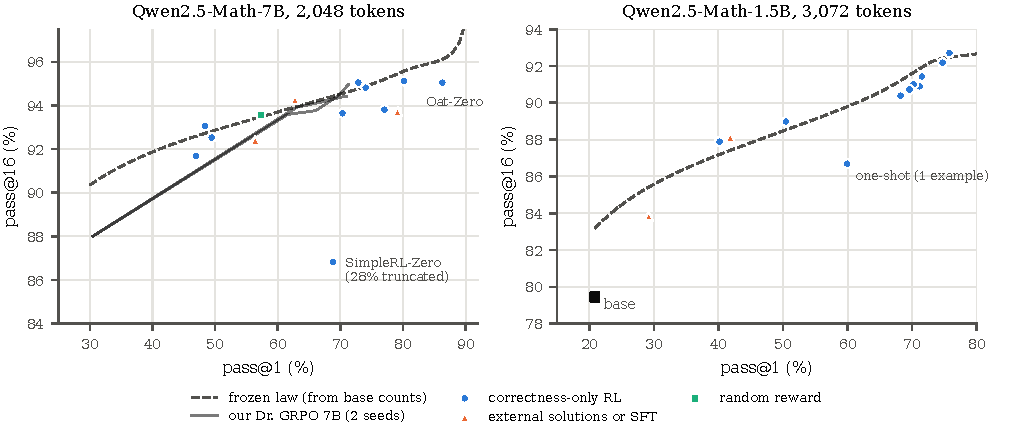
\includegraphics[width=\textwidth]{public_checkpoints.pdf}
\caption{Public checkpoints against the frozen law computed from the base model at the same budget. Left: 7B at
2,048 tokens. Right: 1.5B at 3,072 tokens.}
\label{fig:public}
\end{figure*}

\section{Warm starts lift the curve during early RL}\label{sec:starts}
If RL cannot change the curve, can the starting model? Each start is a small SFT before unchanged Dr.\ GRPO (nominal
dose 25K presented response tokens, AdamW $10^{-5}$, batches of 8; dose chosen on validation after larger doses
moved pass@1 beyond the reference's range). \Cref{tab:starts} lists the registered verdicts.

\textbf{Starts.} \emph{H25}: verified solutions of a stronger model (Qwen2.5-Math-7B-Instruct) to 262 training problems
with at most 4 of 64 base successes; \emph{R25}: the same number of random teacher-covered problems.
\emph{TEACHF} and \emph{SELF}: on 163 hard problems, 256 length-binned pairs of a teacher solution and a verified,
finished base-model solution of the same problem (mean 470 and 466 tokens), so the two differ only in the solution's
source. \emph{CORR}: H25's teacher solutions with the final boxed answer replaced by a wrong one. \emph{FMT}: base
responses with the loss only on box delimiters (its manipulation check failed: boxing did not increase).
\emph{CWS}, \emph{UNI}, \emph{HARD}, \emph{TAIL}: the base model's own verified solutions on 3,795 problems, drawn with
weight $16(1-\hat p_x)^{15}$ (the marginal pass@16 value of \cref{prop:spread}), uniformly, only on $c\le4$ problems,
or uniformly with TailSFT's token filter \citep{malladi2026tailsft}; \emph{TCWS}: coverage weights on teacher
solutions; \emph{TIME}: SELF's stream interleaved during RL (one SFT batch every five steps); \emph{OPD}: on-policy
distillation from the teacher at the same dose \citep{dong2026opd}.

\begin{table}[t]
\caption{Registered warm-start verdicts (1.5B, 1,024 tokens, three RL seeds, RL steps 1--150 where within the
reference's range). Gap: pass@16 at matched pass@1 (points, 95\% interval). Against Dr.\ GRPO unless stated.}
\label{tab:starts}
\centering\small
\resizebox{\columnwidth}{!}{\begin{tabular}{@{}lrl@{}}
\toprule
Start (vs reference) & Gap & Verdict\\
\midrule
H25 (teacher, hard) & $+1.92$ [$+0.68$, $+3.12$] & inconclusive ($<2$)\\
TEACHF (teacher, matched prompts) & $+2.10$ [$+0.86$, $+3.47$] & curve raised\\
CORR (teacher, wrong final box) & $+2.14$ [$+1.04$, $+3.35$] & curve raised\\
H25b (H25, second SFT seed) & $+1.86$ [$+0.71$, $+3.14$] & inconclusive ($<2$)\\
SELF (base's own, matched prompts) & $+1.78$ [$+0.86$, $+2.70$] & inconclusive ($<2$)\\
\midrule
TEACHF vs SELF trajectory & $+1.53$ [$+0.34$, $+2.76$] & teacher beats self\\
CWS vs UNI / HARD / TAIL / SELF & $+0.03$ / $-0.07$ / $+0.47$ / $-0.31$ & none beaten\\
SELF before RL vs TIME (during RL) & $+1.02$ [$+0.29$, $+1.71$] & before better (pre-dose)\\
\quad after TIME's dose completes & $-0.03$ [$-0.62$, $+0.57$] & descriptive\\
OPD vs R25 trajectory & $-1.02$ [$-2.25$, $+0.21$] & inconclusive\\
\bottomrule
\end{tabular}}
\end{table}

\textbf{Teacher content, not labels, timing or weighting.} The cleanest contrast holds prompts and lengths fixed and
changes only who wrote the solutions: teacher solutions beat the base model's own ($+1.53$, all seeds positive).
Corrupting the final answer leaves the effect unchanged (CORR minus H25 $+0.22$, 90\% $[-0.34,+0.82]$), so the carrier
is the reasoning, not the answer key; a second SFT seed reproduces H25 ($-0.06$). Among self-generated starts, coverage
weighting, hard-only selection and TailSFT are indistinguishable (all CWS contrasts within $\pm0.5$; 90\% intervals
within $\pm1$, a descriptive, unadjusted equivalence), and interleaving the same data during RL is equivalent to
applying it before RL once the dose is complete. Coverage-weighted teacher solutions beat coverage-weighted self
solutions by $+1.63$ [$+0.62$, $+2.62$] (not interpreted: support in one seed). On-policy distillation at this dose
gives no gain over plain SFT.

\textbf{A frozen law does not forecast starts.} A per-problem law fitted on Dr.\ GRPO and frozen (\cref{app:law})
forecast $+6.69$ for H25; the observed $+1.92$ gives a residual of $-4.77$ [$-6.57$, $-2.88$]: registered verdict
``forecast fails''. The law describes RL from a given start, not how a start changes the curve.

\textbf{Budget.} At 1,024 tokens the starts truncate 45--48\% of answers. At 2,048 tokens (three seeds), H25's
early-RL gap is $+1.70$ [$+0.50$, $+2.88$] and its start offset $+2.5$ to $+3.3$; over checkpoints 50--150, TEACHF
keeps $+1.72$ [$+0.61$, $+2.83$] while SELF ($-0.03$), CWS ($+0.27$) and UNI ($-0.08$) are near zero (descriptive).

\section{The excursion is transient}\label{sec:persist}
Teacher starts reach pass@1 63--65 by step 150, beyond the 150-step reference's range (about 58), so their late
checkpoints could not be read in \cref{tab:starts}. Three 700-step Dr.\ GRPO replicates (seeds 8--10) reproduce the
150-step references within 2 points of pass@1 and reach pass@1 $65.2$--$65.5$ and pass@16 $88.4$--$89.0$ at step 700.
The registered extension of the H25 and R25 contrasts to these references is not interpretable (support fails in two
seeds; H25's estimate is $+1.54$). Descriptively (\cref{fig:persist}), every start's gap decays. Averaged over seeds,
TEACHF is $+2.1$ at steps 1--10, $+1.3$ at step 50, $+1.2$ at step 100 and $+0.5$ at step 150; CORR $+2.3$, $+1.8$,
$+0.3$, $+0.4$; H25 $+1.8$, $+1.9$, $+0.4$, $+0.4$; SELF $+2.8$, $+0.6$, $+0.6$, $+0.5$. Self starts decay by step 50,
teacher starts by steps 100--150. Teacher starts end where Dr.\ GRPO arrives after about 700 steps, with the same
pass@16: they move faster along the frontier and leave it only transiently. The registered P36 secondary reading
against these references (six arms, Holm) raises no curve; all estimates are $+0.7$ to $+1.6$.

\begin{figure}[t]
\centering
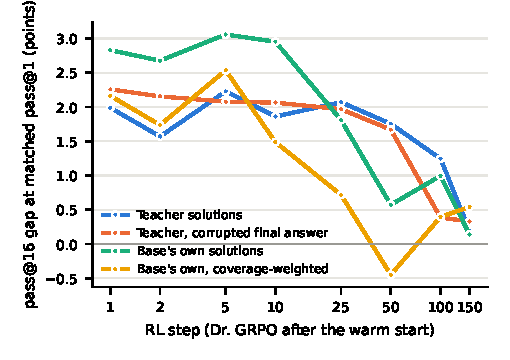
\includegraphics[width=\columnwidth]{start_trajectories.pdf}
\caption{Matched-pass@1 pass@16 gap by RL step after four warm starts, against 700-step Dr.\ GRPO replicates (mean
of seeds 8--10; descriptive). Points lie inside the replicate's pass@1 range in all three seeds.}
\label{fig:persist}
\end{figure}

\section{Where the gains sit}\label{sec:where}
\textbf{Spread, not answer variety.} Across ten RL-side conditions, matched pass@2 gaps are $+0.08$ to $+0.19$ against
$+0.13$ between two Dr.\ GRPO seeds; H25's is $+2.39$ [$+1.97$, $+2.82$] (90\%) and self-generated starts' about
$+1.2$. By \cref{prop:spread}, the coverage gains are a more even distribution of success across problems. Within
problems, the two kinds of start differ: self starts increase distinct incorrect answers ($+1.3$ per problem) while the
teacher start reduces them ($-1.5$); both lower the chance that two incorrect answers coincide. During Dr.\ GRPO itself
(seed 8), that chance rises from 5\% to 14\% while the across-problem variance of success rises from 0.033 to 0.130.

\textbf{Which problems.} An exact decomposition of the matched gap by base-model success count (the reference is
interpolated at overall pass@1 and the same weights are applied within each stratum) shows that self starts' early
gain sits on problems with 1--8 of 64 base successes ($+1.4$ to $+1.7$ of $+1.8$ to $+2.0$ points at steps 1--10) and
is gone by steps 50--150, whereas H25's gain moves toward problems with no base success ($+0.86$ at steps 1--10,
$+1.52$ of $+2.01$ at step 50). Self-generated starts reweight successes the base can already sample, which RL
recovers on its own; teacher reasoning supplies successes on problems the base does not sample, which RL takes longer
to match.

\textbf{Finishing.} Part of RL's own gain is learning to finish an answer: at 1,024 tokens the base leaves 42.5\% of
its answers without a final box; forcing a final answer on the base recovers 16\% of Dr.\ GRPO's pass@1 gain
(\cref{app:finish}).

\section{Related work}\label{sec:related}
\citet{yue2025limit} find base models beating RLVR models at large $k$; the invisible-leash analysis argues RLVR
mostly reweights within the base model's support \citep{wu2025leash}, and RL is reported to squeeze while SFT expands
reasoning trajectories \citep{matsutani2025squeeze}. We test these claims at matched accuracy with registered rules,
across interventions, public checkpoints and warm starts. Diversity-oriented RL methods include pass@$k$ objectives
\citep{walder2025pkpo,chen2025passktraining}, outcome-based exploration \citep{song2025outcome}, entropy control
\citep{cui2025entropy}, rollout scaling and allocation \citep{hu2025brorl,yang2025depth,knapsack2025,yu2026datpo} and
sharpness-aware updates \citep{kim2026flat}; most report fixed-step comparisons, and those we reproduced stay on the
curve. External guidance during RL \citep{yan2025guidance,ma2025relift,li2025questa,zhang2025bread,ding2026lspo} and
self-generated rationalizations \citep{zelikman2022star,zhou2025expo,mahdavi2026splice} inject information the policy
lacks; our warm-start results isolate the content of that information at a fixed dose. Cold-start SFT before RL is
standard \citep{guo2025r1}; on-policy distillation before RL \citep{dong2026opd}, TailSFT \citep{malladi2026tailsft},
mid-training \citep{wang2025octothinker,zhang2025interplay} and distillation \citep{kim2025rlvsdistill} change what RL
can reach; difficulty-aware rejection tuning \citep{tong2024dart} allocates synthesis to hard problems. Budgeted-search
views map RL operating points to base sampling budgets \citep{sun2026boptr}.

\section{Discussion}\label{sec:discussion}
Within the tested settings, RLVR algorithms set how fast a model moves along a coverage-versus-accuracy frontier, the
base model sets the frontier, and warm starts change the position and speed along it, with a transient excursion
whose size depends on whether the start carries reasoning the base cannot sample. A method that durably raises
coverage at matched accuracy would have to change what the policy can reach, not how RL weights what it already
samples. Two open questions are being tested under registered rules \pending{Pre-registration 39 running}: whether a
$k=16$ instrument near ceiling hides RL-side effects at pass@128 on harder held-out problems (OlympiadBench and AIME,
deduplicated against MATH), and whether verified solutions harvested by deep sampling of the base model on problems
it never solves in 64 attempts behave like teacher content.

\section{Limitations}\label{sec:limits}
Models are Qwen2.5-Math 1.5B and 7B on MATH-style problems with binary verification; answer budgets of 512--3,072
tokens are part of the estimand. Bootstrap intervals cover test-problem sampling conditional on the trained seeds.
Average equivalence within $\pm2$ points permits smaller effects; several comparisons are inconclusive or lack
reference support rather than being equivalent. Warm-start arms ran on A100s and the Dr.\ GRPO references on L40S;
within-hardware contrasts (TEACHF vs SELF, CWS vs baselines) are unaffected. The persistence analysis uses three
700-step replicates and is descriptive. pass@16 near 87--89 limits headroom; the base-zero test stratum has 51
problems. A second model family is being prepared.

\bibliography{paper}
\bibliographystyle{icml2026}

\newpage
\appendix
\onecolumn

\section{Registrations and verdicts}\label{app:prereg}
\begin{center}\small
\begin{tabular}{@{}p{0.07\textwidth}p{0.4\textwidth}p{0.48\textwidth}@{}}
\toprule
Reg. & Comparison & Verdict\\
\midrule
9--11 & NSR vs PSR (OLMo, Qwen); noise injection; temperature & Average equivalence; temperature sweep $-1.42$ (90\% $[-2.19,-0.68]$)\\
12, 14 & Coverage-weighted and base-seeded replay; larger groups (G32) & $+1.19$, $+1.02$: below $+2$; G32 exploratory, beyond range\\
16 & Answer budget (check) & Warm-start gain $+4.77\to+2.15$ from 512 to 1,024 tokens: largely a budget effect\\
17 & Frozen per-problem law & RMSE criterion met on three test sets; fails after a warm start\\
18 & Rollout allocation (frontier value, $\E[p(1-p)]$, HORA) & No rule met; forecast not confirmed\\
19, 22 & Human-solution warm starts; human vs self prefixes & Not interpretable (no overlap); prefixes on the curve\\
20, 21 & 7B at 2,048 tokens; 1.5B at 1,024 tokens & 3 of 4 and 4 of 4 contrasts equivalent\\
23, 26 & Minimum-help credit; update-direction, whitening and teacher-gradient pilots & None selected\\
27 & 1,000-step training & Not supported (LH1 borderline)\\
28, 33 & Public checkpoints; 7B sensitivity & No upward departure\\
30 & Teacher warm starts (dose screen; H25, R25; frozen-law forecast) & H25 inconclusive ($+1.92$); R25 not interpreted; forecast fails\\
31 & Flat-RLVR & Average equivalence (both radii)\\
32 & UCB-Con and Batch outcome bonuses & Average equivalence; UCB-Con raises distinct incorrect answers\\
34 & On-policy distillation start & Primary not interpreted; secondary inconclusive ($-1.02$)\\
35, 36 & SELF/TEACHF/CORR/FMT/H25b; CWS, UNI, HARD, TAIL, TCWS, TIME & \Cref{tab:starts}\\
39 & Hard held-out sets, pass@128 re-evaluation, harvest pilot, retention & \pending{running}\\
\bottomrule
\end{tabular}
\end{center}

\section{The frozen per-problem law}\label{app:law}
Each problem's log-odds start at an empirical-Bayes estimate from the base model's 32-sample counts and follow
$\dot\theta_x=p_x(1-p_x)+\tau\frac1N\sum_{x'}p_{x'}(1-p_{x'})$ with $\tau=-0.20$, fitted once on Dr.\ GRPO's 1.5B
checkpoints and frozen; a checkpoint is placed where the law's mean success equals its observed pass@1, and pass@16 is
then a prediction. It describes the curve conditional on pass@1, not training speed.

\section{Finishing}\label{app:finish}
\begin{figure}[H]
\centering
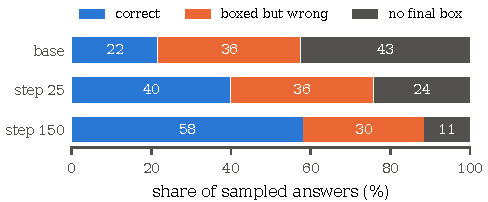
\includegraphics[width=0.55\textwidth]{finishing.pdf}
\caption{Answers of the 1.5B base and Dr.\ GRPO (seed 8) at steps 25 and 150 at 1,024 tokens: correct, boxed but wrong,
and without a final box.}
\end{figure}
Between the base and step 25, correct answers rise by 18.4 points while unfinished answers fall by 18.3. Appending
``Final answer: \textbackslash boxed\{'' to unfinished base samples and decoding 32 greedy tokens raises pass@1 from
22.0 to 27.7 (22.3 with the same extra tokens and no cue).

\section{Long references}\label{app:long}
The 700-step replicates B1kL8--10 (L40S, the B1k recipe) reach pass@1/pass@16 of $39.2/84.9$, $51.7/85.7$,
$56.4/86.3$, $58.3/86.7$ (seed 8) at steps 25, 50, 100, 150, against $40.0/85.1$, $52.6/86.1$, $56.4/87.4$, $58.1/86.5$
for B1k8; at steps 200--700 seed 8 reaches $59.7/87.6$, $60.9/87.8$, $61.8/87.9$, $63.2/88.1$, $63.7/87.7$, $65.5/88.5$.

\end{document}
